% \documentclass[10pt]{beamer}
\documentclass[9pt, aspectratio=169]{beamer}
\usepackage[utf8]{inputenc}
\usepackage[T1]{fontenc}
%\usepackage{lmodern}
\usepackage{amsfonts,amssymb,amsmath}
\usepackage[english]{babel}
\usetheme{Frankfurt}

\usepackage{csquotes}
\usepackage{setspace}

\usepackage{colortbl}
\usepackage{tabularx}
\renewcommand\tabularxcolumn[1]{m{#1}}

\setbeamertemplate{navigation symbols}{}
\setbeamertemplate{footline}[frame number]{}

% --- Tickz
\usepackage{physics}
\usepackage{amsmath}
\usepackage{tikz}
\usepackage{mathdots}
\usepackage{yhmath}
\usepackage{cancel}
\usepackage{color}
\usepackage{siunitx}
\usepackage{array}
\usepackage{multirow}
\usepackage{amssymb}
\usepackage{gensymb}
\usepackage{tabularx}
\usepackage{extarrows}
\usepackage{booktabs}
\usetikzlibrary{fadings}
\usetikzlibrary{patterns}
\usetikzlibrary{shadows.blur}
\usetikzlibrary{shapes}

% ---------

\usepackage{booktabs}
\usepackage{setspace}
\usepackage{amssymb}
\usepackage{adjustbox}
\usepackage{pifont}
\usepackage[inkscapeformat=png]{svg}
\usepackage{graphicx}
\usepackage{times}
\setbeamertemplate{caption}[numbered]
% \setbeamertemplate{bibliography item}{[\theenumiv]}
\setbeamertemplate{bibliography item}[text]

\setbeamerfont{bibliography item}{size=\tiny}
\setbeamerfont{bibliography entry author}{size=\tiny}
\setbeamerfont{bibliography entry title}{size=\tiny}
\setbeamerfont{bibliography entry location}{size=\tiny}
\setbeamerfont{bibliography entry note}{size=\tiny}

% \setbeamerfont{frametitle}{size=\large}

\usepackage{caption}
\usepackage{float}
\usepackage{xcolor}
\usepackage{listings}

\definecolor{codegreen}{rgb}{0,0.6,0}
\definecolor{codegray}{rgb}{0.5,0.5,0.5}
\definecolor{codepurple}{rgb}{0.58,0,0.82}
\definecolor{backcolour}{rgb}{0.95,0.95,0.92}
 
\lstdefinestyle{mystyle}{
    backgroundcolor=\color{backcolour},   
    commentstyle=\color{codegreen},
    keywordstyle=\color{magenta},
    numberstyle=\tiny\color{codegray},
    stringstyle=\color{codepurple},
    basicstyle=\footnotesize,
    breakatwhitespace=false,         
    breaklines=true,                 
    captionpos=b,                    
    keepspaces=true,                 
    numbers=left,                    
    numbersep=5pt,                  
    showspaces=false,                
    showstringspaces=false,
    showtabs=false,                  
    tabsize=2
}
 
\lstset{style=mystyle}

\usepackage{ragged2e}
\setbeamercolor{section in foot}{fg=white,bg=darkorange}
\setbeamercolor{subsection in foot}{fg=white,bg=darkorange}
\setbeamercolor{frametitle}{fg=white, bg=darkorange}
\setbeamercolor{title}{fg=white, bg=darkorange}
\setbeamercolor{frame}{bg=darkorange}
\setbeamercolor{block title}{bg=darkorange,fg=white}

\setbeamercolor{item}{fg=darkorange}

% \definecolor{darkorange}{rgb}{0.81, 0.52, 0.05}
\definecolor{darkorange}{rgb}{1,0.5,0}
\definecolor{darkorange2}{rgb}{1, 0.64, 0.2}
\definecolor{honeydew}{rgb}{1, 0.85, 0.45}


\newenvironment{variableblock}[3]{%
  \setbeamercolor{block body}{#2}
  \setbeamercolor{block title}{#3}
  \begin{block}{#1}}{\end{block}}

\newenvironment{prosblock}[1]{%
  % \setbeamercolor{block body}{bg=blue,fg=white}
  \setbeamercolor{block title}{bg=blue,fg=white}
  \begin{block}{#1}}{\end{block}}

\newenvironment{consblock}[1]{%
  % \setbeamercolor{block body}{bg=red,fg=white}
  \setbeamercolor{block title}{bg=red,fg=white}
  \begin{block}{#1}}{\end{block}}

\newcommand{\cmark}{\ding{51}}%
\newcommand{\xmark}{\ding{55}}%

\renewcommand{\arraystretch}{1.5}

\usepackage{tabularray}\UseTblrLibrary{varwidth}
\usepackage{xcolor}
\def\BibTeX{{\rm B\kern-.05em{\sc i\kern-.025em b}\kern-.08em
    T\kern-.1667em\lower.7ex\hbox{E}\kern-.125emX}}
\usepackage{cite}
\usepackage{amsmath}
\newcommand{\probP}{\text{I\kern-0.15em P}}
\usepackage{etoolbox}
\patchcmd{\thebibliography}{\section*{\refname}}{}{}{}

\setlength\tabcolsep{0.5pt}

% for video embedding
% %%%%%%%%%%%%%%%%%%%%%%%%%%%%%%%%%%%%%%%%%%%%%%%%%%%%%%%%%%%%%%%%%%%%%%%%%%%%%%
% \embedvideo{<poster or text>}{<video file (MP4+H264)>}
% \embedvideo*{...}{...}                     % auto-play
%%%%%%%%%%%%%%%%%%%%%%%%%%%%%%%%%%%%%%%%%%%%%%%%%%%%%%%%%%%%%%%%%%%%%%%%%%%%%%

\usepackage[bigfiles]{pdfbase}
\ExplSyntaxOn
\NewDocumentCommand\embedvideo{smm}{
  \group_begin:
  \leavevmode
  \tl_if_exist:cTF{file_\file_mdfive_hash:n{#3}}{
    \tl_set_eq:Nc\video{file_\file_mdfive_hash:n{#3}}
  }{
    \IfFileExists{#3}{}{\GenericError{}{File~`#3'~not~found}{}{}}
    \pbs_pdfobj:nnn{}{fstream}{{}{#3}}
    \pbs_pdfobj:nnn{}{dict}{
      /Type/Filespec/F~(#3)/UF~(#3)
      /EF~<</F~\pbs_pdflastobj:>>
    }
    \tl_set:Nx\video{\pbs_pdflastobj:}
    \tl_gset_eq:cN{file_\file_mdfive_hash:n{#3}}\video
  }
  %
  \pbs_pdfobj:nnn{}{dict}{
    /Type/RichMediaInstance/Subtype/Video
    /Asset~\video
    /Params~<</FlashVars (
      source=#3&
      skin=SkinOverAllNoFullNoCaption.swf&
      skinAutoHide=true&
      skinBackgroundColor=0x5F5F5F&
      skinBackgroundAlpha=0
    )>>
  }
  %
  \pbs_pdfobj:nnn{}{dict}{
    /Type/RichMediaConfiguration/Subtype/Video
    /Instances~[\pbs_pdflastobj:]
  }
  %
  \pbs_pdfobj:nnn{}{dict}{
    /Type/RichMediaContent
    /Assets~<<
      /Names~[(#3)~\video]
    >>
    /Configurations~[\pbs_pdflastobj:]
  }
  \tl_set:Nx\rmcontent{\pbs_pdflastobj:}
  %
  \pbs_pdfobj:nnn{}{dict}{
    /Activation~<<
      /Condition/\IfBooleanTF{#1}{PV}{XA}
      /Presentation~<</Style/Embedded>>
    >>
    /Deactivation~<</Condition/PI>>
  }
  %
  \hbox_set:Nn\l_tmpa_box{#2}
  \tl_set:Nx\l_box_wd_tl{\dim_use:N\box_wd:N\l_tmpa_box}
  \tl_set:Nx\l_box_ht_tl{\dim_use:N\box_ht:N\l_tmpa_box}
  \tl_set:Nx\l_box_dp_tl{\dim_use:N\box_dp:N\l_tmpa_box}
  \pbs_pdfxform:nnnnn{1}{1}{}{}{\l_tmpa_box}
  %
  \pbs_pdfannot:nnnn{\l_box_wd_tl}{\l_box_ht_tl}{\l_box_dp_tl}{
    /Subtype/RichMedia
    /BS~<</W~0/S/S>>
    /Contents~(embedded~video~file:#3)
    /NM~(rma:#3)
    /AP~<</N~\pbs_pdflastxform:>>
    /RichMediaSettings~\pbs_pdflastobj:
    /RichMediaContent~\rmcontent
  }
  \phantom{#2}
  \group_end:
}
\ExplSyntaxOff
%%%%%%%%%%%%%%%%%%%%%%%%%%%%%%%%%%%%%%%%%%%%%%%%%%%%%%%%%%%%%%%%%%%%%%%%%%%%%%

\begin{document}

\author{\textbf{Julien Soulé}, Jean-Paul Jamont, Michel Occello, Paul Théron, Louis-Marie Traonouez}

\title{\textbf{Towards a Multi-Agent Simulation of Cyber-attackers and Cyber-defenders Battles}}

\subtitle{SMC 2023 Presentation}

% \logo{
\includegraphics[scale=0.01]{figures/grenoble-inp_logo.png}}

\institute{\footnotesize \textit{University Grenoble Alpes, Grenoble
INP, LCIS, 26000, Valence, France \\
julien.soule@lcis.grenoble-inp.fr}}

\date{\textit{\footnotesize \today}}

%\subject{}
\setbeamercovered{transparent}
%\setbeamertemplate{navigation symbols}{}
\begin{frame}[plain]
	\maketitle\vspace{-0.8cm}
	\begin{figure}[ht!]
		\centering
            
\includegraphics[height=0.8cm]{figures/la-ruche_logo.png}
            \hspace{0.8cm}
            
\includegraphics[height=0.8cm]{figures/lcis_logo.png}
            \hspace{0.8cm}
		
\includegraphics[height=0.8cm]{figures/grenoble-inp_logo.png}
            \hspace{0.8cm}
            
\includegraphics[height=0.8cm]{figures/uga_logo.jpg}
	\end{figure}
\end{frame}

% \begin{frame}{Content}
%   \tableofcontents
% \end{frame}

\AtBeginSection[]{
	\begin{frame}
		\frametitle{}
		\tableofcontents[currentsection]
	\end{frame}
}

%%%%%%%%%%%%%%%%%%%%%%%%%%%%%%%%%%%%

	\section{Introduction}
	\begin{frame}[allowframebreaks]{Introduction}

	   \begin{block}{AICA: Autonomous Intelligent Cyberdefense Agent \cite{theron_autonomous_2021}}

            An agent theorized by « IST-152 NATO » between 2016-2019 that is to be deployed on networked nodes to:
 
	       \begin{itemize}
                \item Detect, identify and characterize anomalies/attacks
                \item Plan and execute countermeasures
                \item Communicate with C2, operators\dots
                \item Being autonomous, stealthy, inter-operable, able to learn
		\end{itemize}

        \end{block}

        \begin{block}{MASCARA: Multi Agent System Centric AICA Reference Architecture \cite{theron_autonomous_2021}}
            \begin{itemize}
                \item A multi-agent vision of a decentralized and distributed AICA;
                \item A set of collaborative cyber-defenders fighting back against cyber-attacker(s) deployed over a networked system.
            \end{itemize}
        \end{block}

        \begin{alertblock}{Main concerns}
            No available consistent, clear and general framework to deal with cyber-defenders fighting against cyber-attackers in a networked system:
            \begin{itemize}
                \item Need to clarify how agents, environment and their interactions should be envisioned consistently;
                \item Need to assess collective cyber-defense experimentally through various criteria.
            \end{itemize}

        \end{alertblock}

        \begin{block}{Intended contributions}
            \begin{itemize}
                \item A formal model for cyber-defenders fighting against cyber-attackers in a networked system;
                \item A simulation tool to assess the efficiency of cyber-defenders / cyber-attackers collective actions for various attack scenarios.
            \end{itemize}
        \end{block}
 
	\end{frame}
% \AtBeginSection[]{
%     \begin{frame}
%         \frametitle{}
%         \tableofcontents[currentsection]
%     \end{frame}
% }

%%%%%%%%%%%%%%%%%%%%%%%%%%%%%%%%%%%%

\section{Theoretical background: MARL \& OM}



\subsection{(G1) Multi-Agent Reinforcement Learning}

\begin{frame}{(G1) Multi-Agent Reinforcement Learning}{MARL basics}

    \begin{columns}

        \hspace{-2ex}

        \begin{column}{0.4\textwidth}

            \begin{figure}
                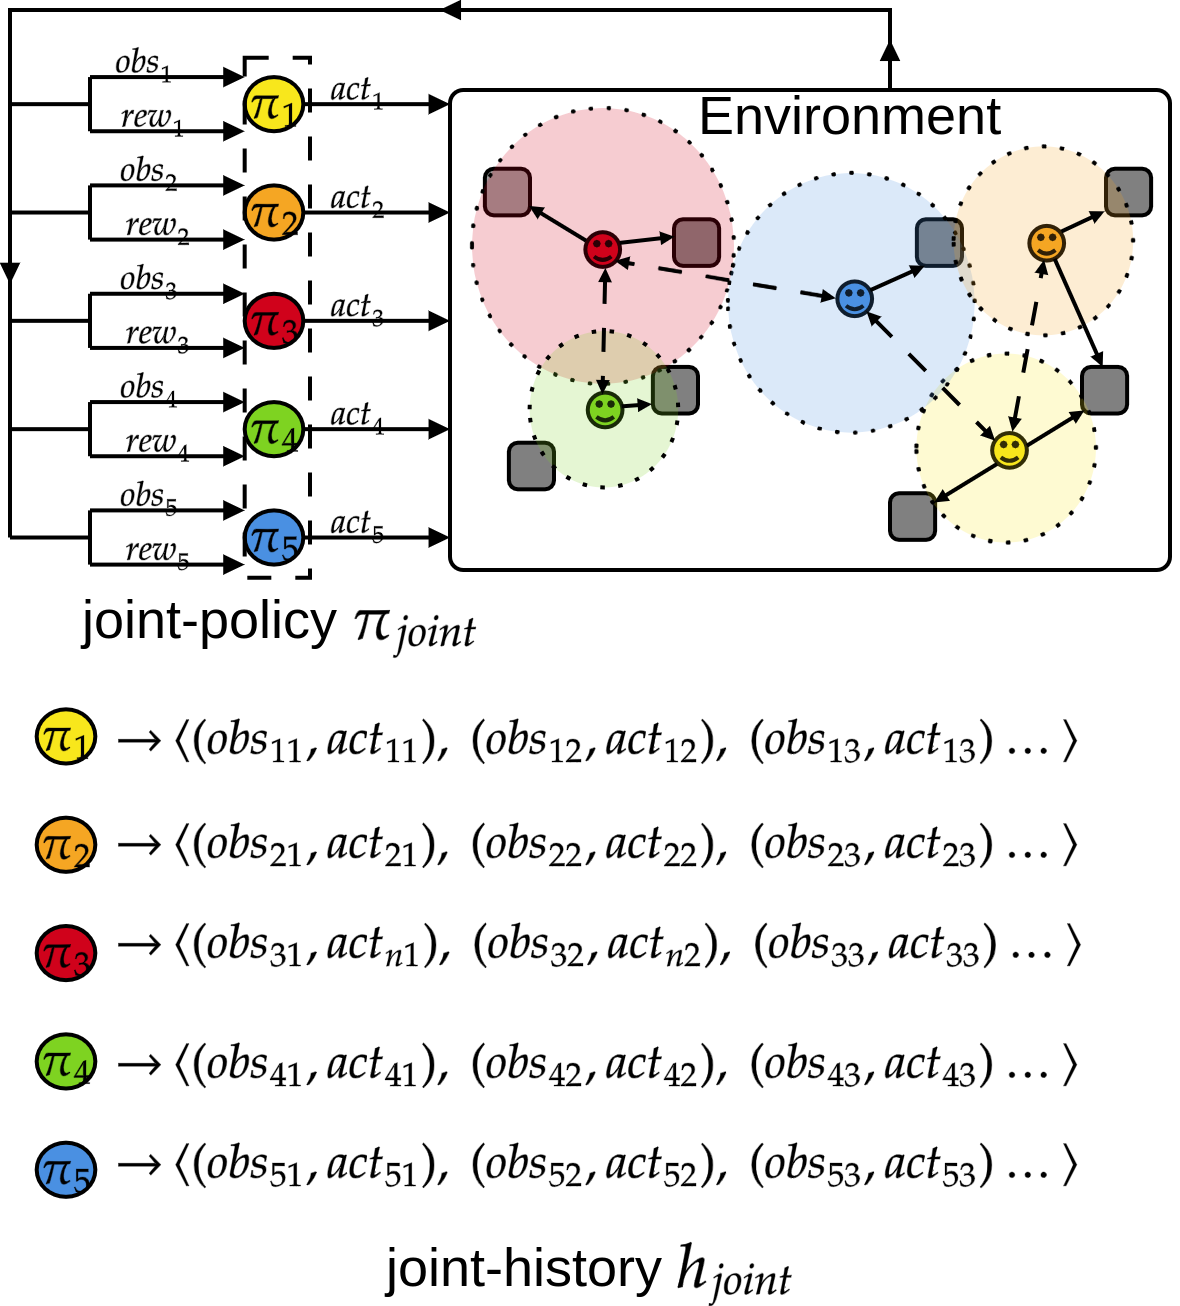
\includegraphics[width=\linewidth]{figures/marl_basics.png}
            \end{figure}

        \end{column}

        \begin{column}{0.7\textwidth}
            \vspace{-2ex}

            \begin{center}
                \begin{minipage}{0.95\linewidth}
                    \centering
                    \begin{block}{Markovian models for MARL: Dec-POMDP}
                        {\small
                            Decentralized Partially Observable Markov Decision Process (Dec-POMDP)~\cite{Oliehoek2016}
                            \begin{itemize}
                                \item considers multiple agents in a similar MAS fashion
                                \item stochastic processes for uncertainty in environmental changes including observations;
                                \item reward function is common to agents which fosters training for collaborative oriented actions~\cite{Beynier2013}
                            \end{itemize}
                        }
                        \

                        { \scriptsize

                        $(S,\{A_i\},T,R,\{\Omega_i\},O,\gamma)$ , where
                        \begin{itemize}
                            \item $S = \{s_1, ..s_{|S|}\}$: The set of the possible states;
                            \item $A_{i} = \{a_{1}^{i},..,a_{|A_{i}|}^{i}\}$: The set of the possible actions for agent $i$;
                            \item $T$ so that $T(s,a,s') = \probP{(s'|s,a)}$ : The set of conditional transition probabilities;
                            \item $R: S \times A \times S \rightarrow \mathbb{R}$: The reward function
                            \item $\Omega_{i} = \{o_{1}^{i},..,o_{|\Omega_{i}|}^{i}\}$: The set of observations for agent $ag_i$;
                            \item $O$ so that $O(s',a,o) = \probP{(o|s',a)}$ : The set of conditional observation probabilities;
                            \item $\gamma \in [0,1]$, the discount factor.
                        \end{itemize}

                        }

                    \end{block}

                \end{minipage}
            \end{center}

        \end{column}

    \end{columns}

\end{frame}

\begin{frame}{(G1) Multi-Agent Reinforcement Learning}{MARL for solving/designing}

    \begin{block}{MARL for methodological purpose in literature?}

        Effective joint-policies but \textbf{not explicitly} specified/understandable
        $\Longrightarrow$ Few related works
            {\small
                \begin{itemize}
                    \item Kazhdan et. al.~\cite{Kazhdan2020} proposed means to extract symbolic models $\rightarrow$ \textbf{not scalable};
                    \item Wang et. al.~\cite{Wang2020}: introduced a role-oriented MARL approach $\rightarrow$ \textbf{roles only};
                    \item Zheng et. al.~\cite{Zheng2018} presented a platform for MARL $\rightarrow$ \textbf{empirical tools}.
                \end{itemize}
            }
    \end{block}

    \begin{block}{Solving a Dec-POMDP}
        \begin{itemize}
            \item \textbf{solving}: finding a joint policy $\pi_{joint,i} \in \Pi_{joint}$ maximizing cumulative reward over time;
            \item \textbf{sub-optimally solving}: finding a joint policy $\pi_{joint,i} \in \Pi_{joint}$ so that expected cumulative reward over time at least at $s \in \mathbb{R}$.
        \end{itemize}
    \end{block}

    \begin{exampleblock}{Examples of MARL Algorithms}
        {\footnotesize

            \centering
            \begin{minipage}{0.5\textwidth}
                \centering
                \begin{itemize}
                    \item \textbf{Independent Learning}: IQL, IDQN
                    \item \textbf{Centralized Training, Decentralized Execution}: MADDPG, COMA, VDN
                \end{itemize}
            \end{minipage}\hfill
            \begin{minipage}{0.5\textwidth}
                \centering
                \begin{itemize}
                    \item \textbf{Cooperative MARL}: QMIX, MAPPO
                    \item \textbf{Hierarchical MARL}: Feudal Networks, Hierarchical Actor-Critic
                \end{itemize}
            \end{minipage}\hfill
        }
    \end{exampleblock}

\end{frame}



\subsection{Organizational Model}

\begin{frame}{(G2) Organizational Model}{$\mathcal{M}OISE^+$}

    \begin{figure}
        \centering
        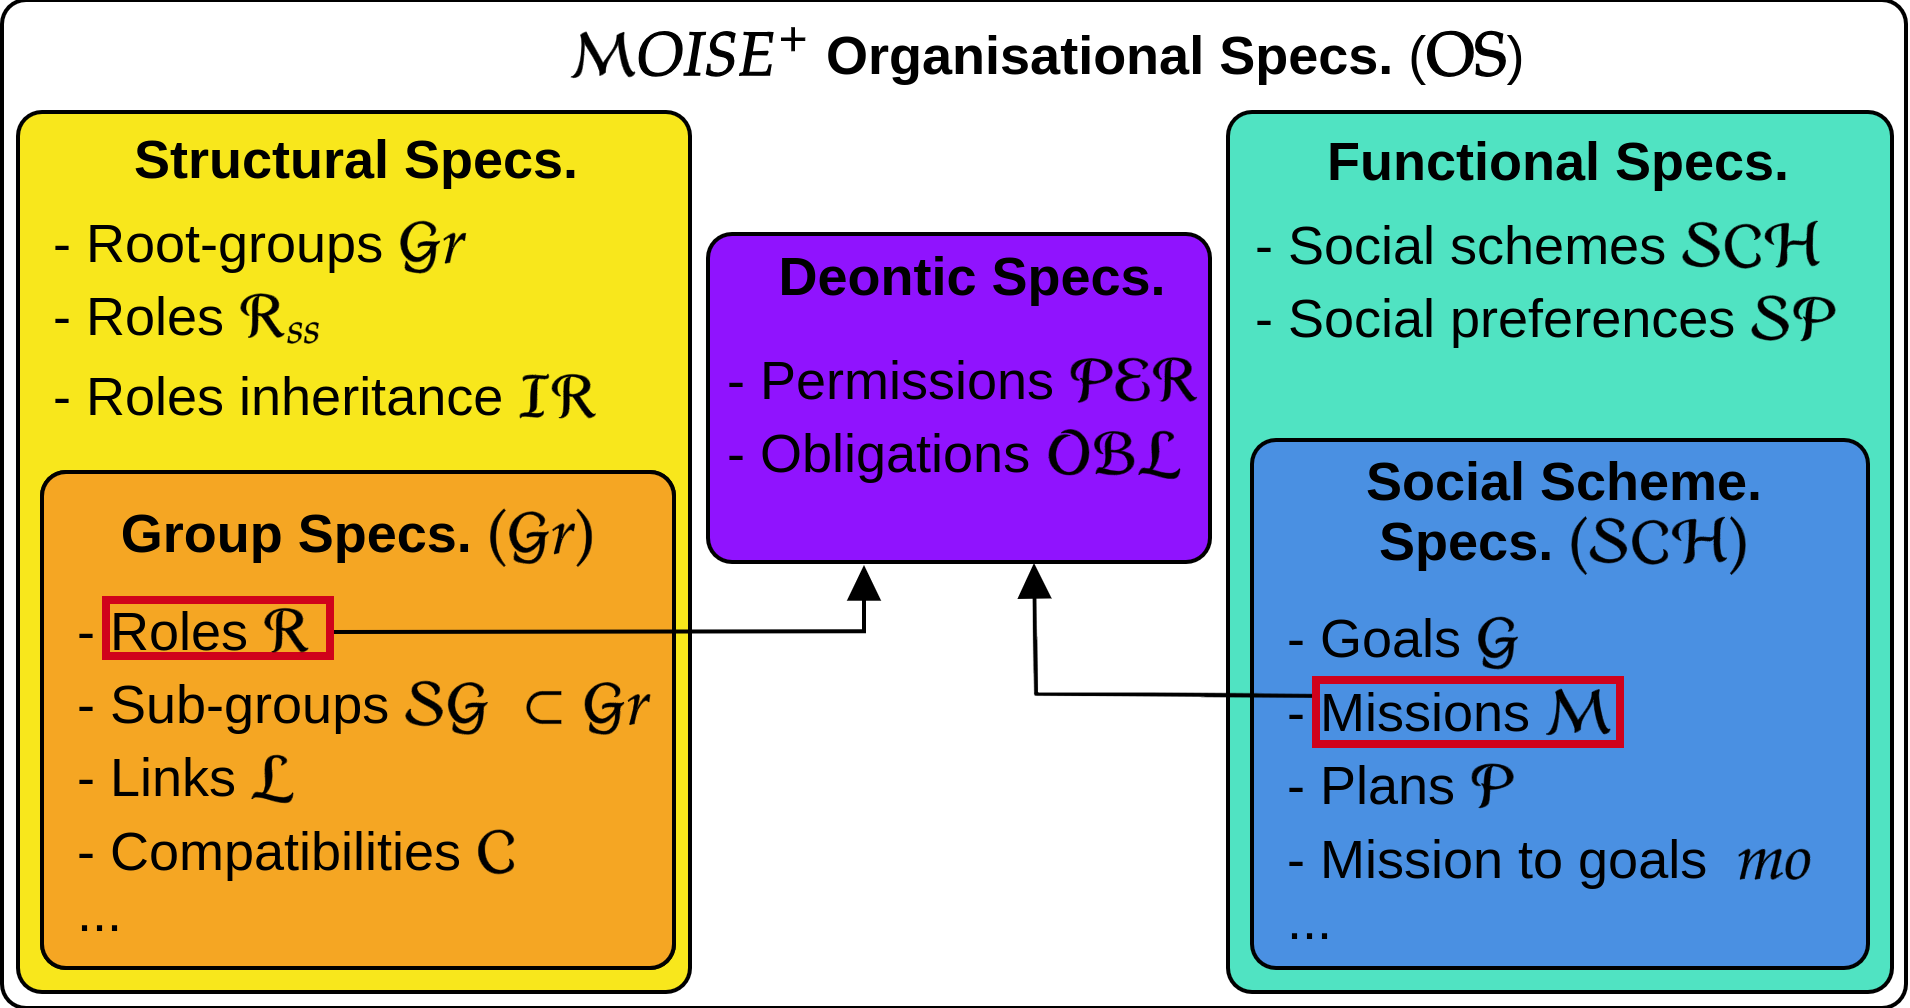
\includegraphics[width=0.75\linewidth]{figures/moise_model.png}
    \end{figure}

    \begin{spacing}{0.25}
        {\tiny Hübner, J. F., Sichman, J. S., and Boissier, O. (2002).
            A model for the structural, functional, and deontic specification of
            organizations in multiagent systems.
            In Bittencourt, G. and Ramalho, G. L., editors, Proceedings of the 16th Brazilian Symposium on Artificial Intelligence (SBIA’02), volume 2507 of LNAI, pages 118–128, Berlin. Springer.}
    \end{spacing}

\end{frame}

\begin{frame}{(G2) Organizational Model}{\textit{Soccer team example}}

    \vspace{-2.5ex}

    \begin{columns}
        \hspace{-16ex}
        \begin{column}{0.5\textwidth}
            \centering
            \begin{figure}[H]
                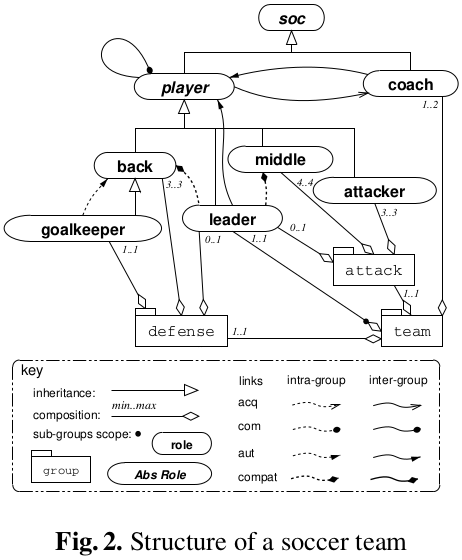
\includegraphics[width=0.7\textwidth]{figures/soccer_ss.png}
                \caption*{Structural Specifications}
            \end{figure}
        \end{column}
        \hspace{-20ex}
        \begin{column}{0.5\textwidth}
            \centering
            \begin{figure}[H]
                \centering
                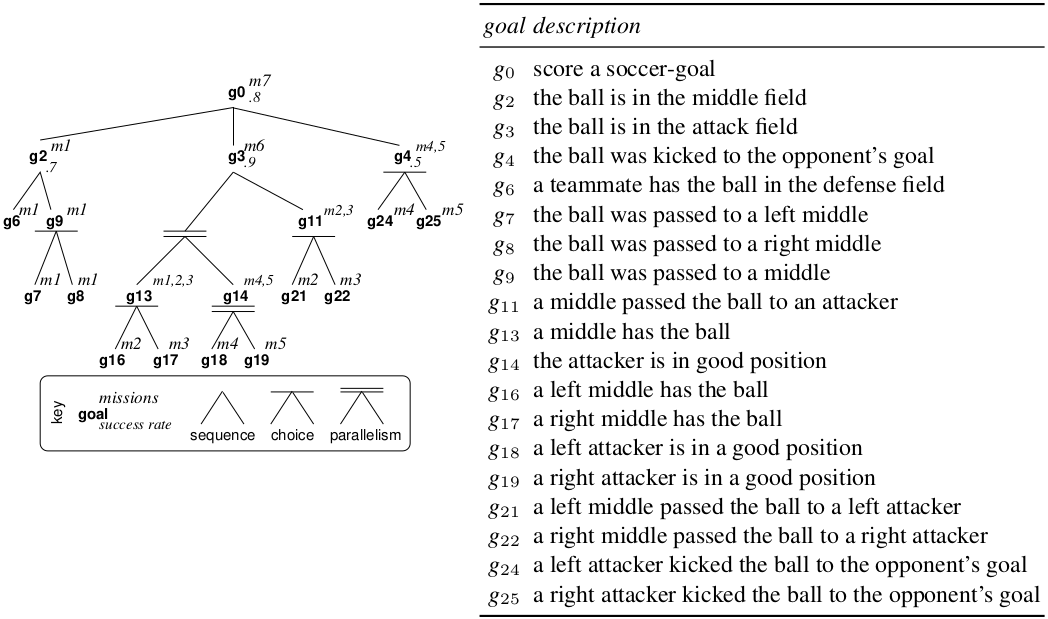
\includegraphics[width=1.2\textwidth]{figures/soccer_fs.png}
                \caption*{Functional Specifications}
            \end{figure}
        \end{column}
    \end{columns}

    % \begin{minipage}{0.5\textwidth}
    %     \centering

    % \end{minipage}\hfill
    % %
    % \begin{minipage}{0.5\textwidth}
    %     \centering

    % \end{minipage}\hfill

    \ \\

    \begin{minipage}{\textwidth}
        \centering
        \begin{figure}[H]
            \centering
            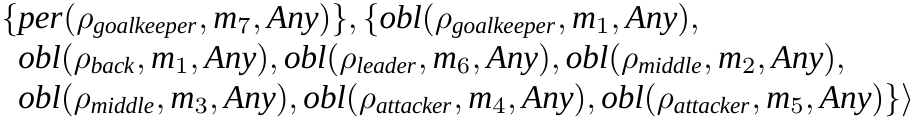
\includegraphics[width=0.4\linewidth]{figures/soccer_ds.png}
            \caption*{Deontic Specifications}
        \end{figure}
    \end{minipage}

    % \begin{figure}
    %     \centering
    %     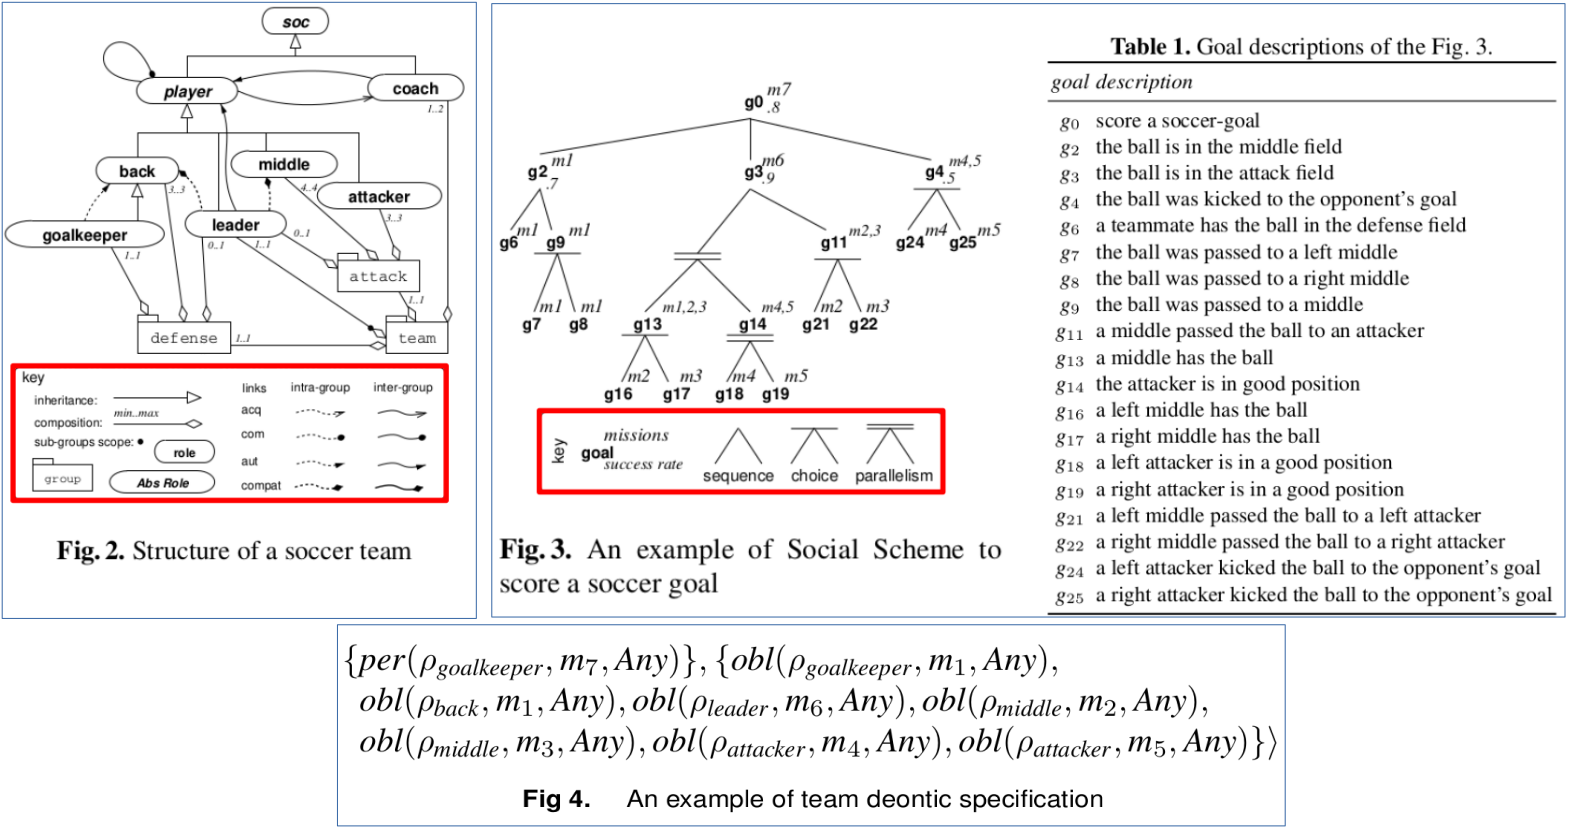
\includegraphics[width=\linewidth]{figures/soccer_os.png}
    % \end{figure}

\end{frame}

% \AtBeginSection[]{
%     \begin{frame}
%         \frametitle{}
%         \tableofcontents[currentsection]
%     \end{frame}
% }

%%%%%%%%%%%%%%%%%%%%%%%%%%%%%%%%%%%%

\section{Preuve de Concept sur exemple}

\begin{frame}[fragile]{Preuve de Concept sur exemple}{Initialisation}

    \begin{columns}

        \begin{column}{0.6\textwidth}

            \begin{enumerate}
                \item Initialiser environment PettingZoo
                \item Mapping observation labels
            \end{enumerate}
    
\begin{lstlisting}[language=Python,basicstyle=\scriptsize]
from custom_envs.movingcompany import moving_company_v0
from prahom_wrapper.prahom_wrapper import prahom_wrapper

env = moving_company_v0.parallel_env(render_mode="human")

label_to_obs = {
    "empty_corridor_0": [0,1,0,0,1,0,0,1,0],
    "empty_corridor_1": [0,1,0,0,2,0,0,1,0],
    "empty_corridor_2": [0,1,0,0,3,0,0,1,0],
}
\end{lstlisting}
    
        \end{column}
    
        \begin{column}{0.4\textwidth}
            \centering
            \begin{figure}
                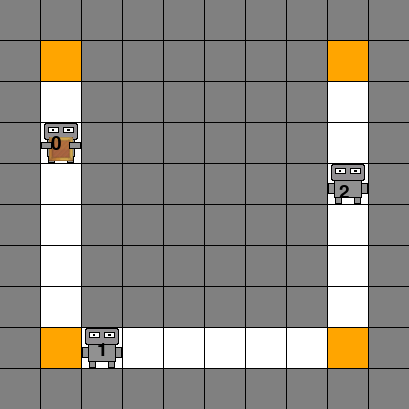
\includegraphics[width=\linewidth]{figures/moving_company_v0.png}
                \caption{Exemple de rendu graphique de l'environment \textquote{Moving Company}}
            \end{figure}
        \end{column}
    
    \end{columns}


\end{frame}


\begin{frame}

    % Boucle pour afficher toutes les images de frame000.png à frame099.png
    \foreach \i in {00, 01, 02, 03, 04, 05, 06, 07, 08, 09, 10, 11, 12, 13, 14, 15, 16, 17, 18, 19, 20} {
    
        \begin{onlyenv}<\i>
        % \begin{frame}[plain]
            \frametitle{Exemple : Moving Company après entrainement}
            \centering
            \includegraphics[width=0.5\textwidth]{figures/mcy_frames/frame_\i_delay-0.01s.png}
        % \end{frame}
    
        \end{onlyenv}
    
    }
    
\end{frame}


\begin{frame}[fragile]{Preuve de Concept sur exemple}{}

    \begin{columns}

        \begin{column}{0.6\textwidth}
    
            \textbf{Phase 1 : Modélisation}
    
            \begin{itemize}
                \item Développer manuellement un environnement simulé ($1.1$) où les agents doivent coopérer pour atteindre un objectif ($1.2$);
                \item Peut définir le comportement attendu des rôles sous forme d'historiques;
                \item Peut contraindre les agents à des rôles ($1.3$).
            \end{itemize}
    
            \begin{lstlisting}[language=Python,basicstyle=\scriptsize]
org_model = organizational_model(
    structural_specifications=ss(
        roles={ "role_0": history_subset(pattern="[o0,a1](1,4),[o1,a2](1,2)")},
        role_inheritance_relations=None, root_groups=None),
    
    functional_specifications=fs(
        social_scheme=sch(
            goals={"goal_0": history_subset(pattern="[#Any](0,*),[obs_goal_0]")},missions=["mission_0"], goals_structure=None,mission_to_goals={"mission_0": ["goal_0"]},mission_to_agent_cardinality=None),
        social_preferences=None),

    deontic_specifications={
        "role_0": {("mission_0", "Any"): ["agent_0", "agent_2"]}})\end{lstlisting}

        \end{column}
    
        \begin{column}{0.4\textwidth}
            \centering
            \adjustbox{trim={0.\width} {0.82\height} {0.\width} {0.\height}, clip}{%
                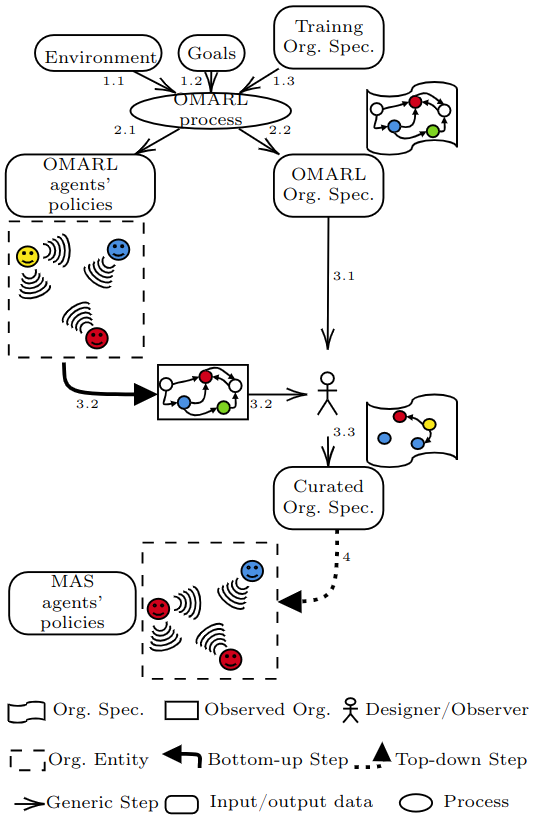
\includegraphics[width=1.2\linewidth]{figures/AOMEA_illustrative_view}
            }
        \end{column}
    
    \end{columns}
    
    
    \end{frame}
    
    
    \begin{frame}[fragile]{Preuve de Concept sur exemple}{}
    
    \begin{columns}
    
        \begin{column}{0.6\textwidth}
    
            \textbf{Phase 2 : Résolution}
    
            \begin{itemize}
                \item Algorithme MARL orienté organisation (OMARL) : processus MARL enrichi avec le modèle organisationnel;
                \item Résoudre en respectant les historiques contraints des rôles ($2.1$);
                \item Obtient l'OS associé ($2.2$)
            \end{itemize}

            \begin{lstlisting}[language=Python,basicstyle=\scriptsize]
pz_env.train_under_constraints(
    obs_act_to_labels=oal,
    constraint_integration_mode="CORRECT",algorithm_configuration="default_MAPPO"
    osh_model_constraint=osh_model)
            \end{lstlisting}

        \end{column}
    
        \begin{column}{0.4\textwidth}
            \centering
            \adjustbox{trim={0.\width} {0.56\height} {0.\width} {0.\height}, clip}{%
                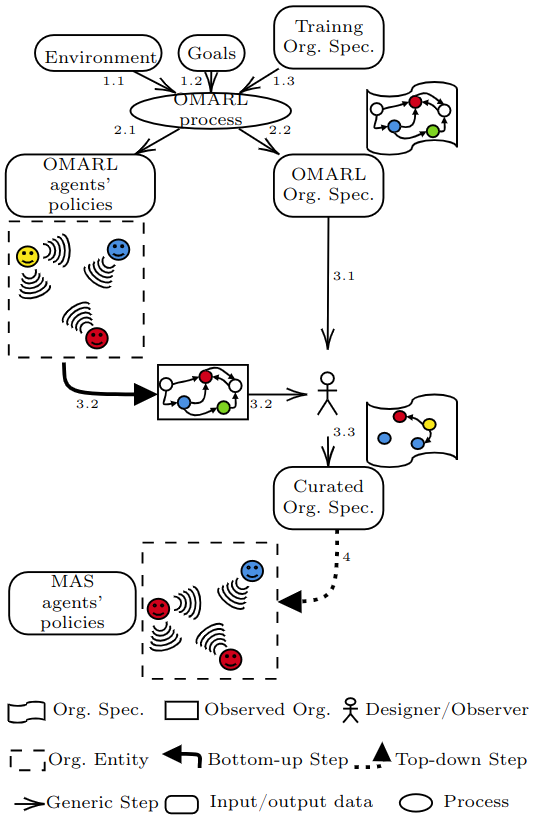
\includegraphics[width=1.2\linewidth]{figures/AOMEA_illustrative_view}
            }
        \end{column}
    
    \end{columns}
    
    \end{frame}
    
    \begin{frame}[fragile]{Preuve de Concept sur exemple}
    
    \begin{columns}
    
        \begin{column}{0.6\textwidth}
    
            \textbf{Phase 3 : Analyse}
    
            \begin{itemize}
                \item Les concepteurs observent les politiques des agents entraînés ($3.2$);
                \item Les concepteurs observent les SO calculés ($3.1$) : comprendre comment ils atteignent l'objectif;
                \item Les concepteurs obtiennent des indications de conception pour un SMA atteignant l'objectif : OS corrigé ($3.3$).
            \end{itemize}

            \begin{lstlisting}[language=Python,basicstyle=\scriptsize]
pz_env.generate_organizational_specifications(use_kosia=False, use_gosia=True,gosia_configuration={"generate_figures": True})
            \end{lstlisting}

        \end{column}
    
        \begin{column}{0.4\textwidth}
            \centering
            \adjustbox{trim={0.\width} {0.35\height} {0.\width} {0.188\height}, clip}{%
                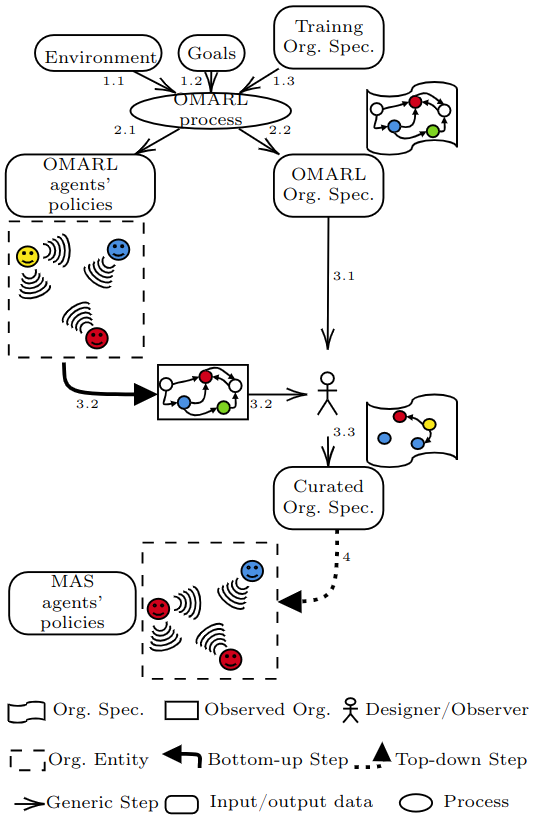
\includegraphics[width=1.2\linewidth]{figures/AOMEA_illustrative_view}
            }
        \end{column}
    
    \end{columns}
    
    \end{frame}
    
    \begin{frame}[fragile]{Preuve de Concept sur exemple}

        \begin{figure}
            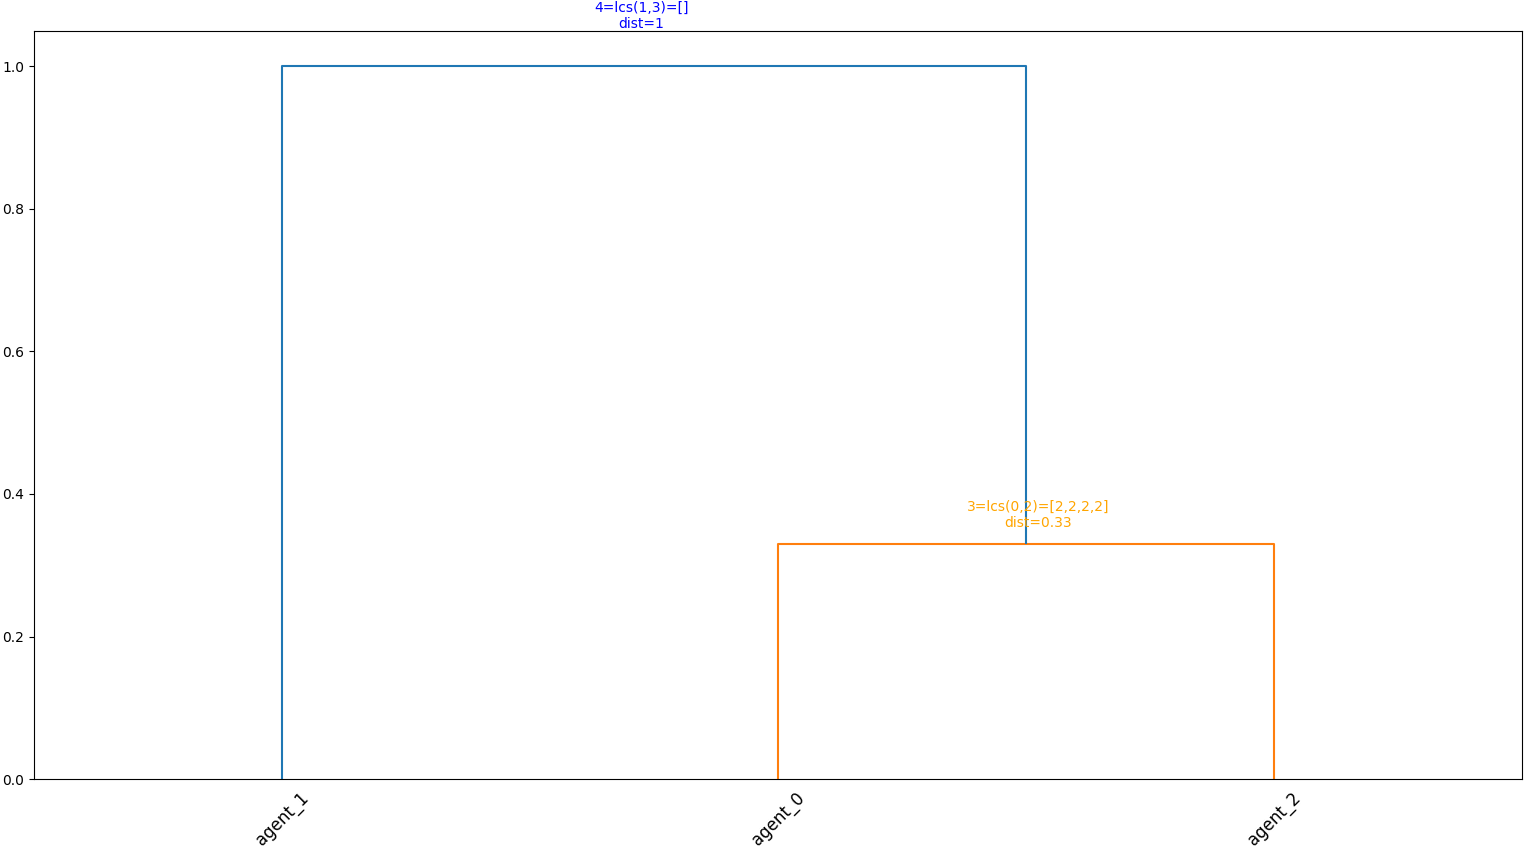
\includegraphics[width=0.7\linewidth]{figures/role_clustering.png}
            \caption*{Exemple de Dendrogramme obtenu après \textit{Hierarchical Clustering}}
        \end{figure}

    \end{frame}
        

    \begin{frame}[fragile]{Preuve de Concept sur exemple}
    
    \begin{columns}
    
        \begin{column}{0.6\textwidth}
    
            \textbf{Phase 4 : Développement}
    
            \begin{itemize}
                \item Les concepteurs observent l'OS corrigé pour implémenter un SMA;
                \item Développement d'un SMA régulier, traitant ainsi les questions de sécurité;
                \item Évaluation du SMA implémenté dans des simulations.
            \end{itemize}
    
        \end{column}
    
        \begin{column}{0.4\textwidth}
            \centering
            \adjustbox{trim={0.\width} {0.15\height} {0.\width} {0.57\height}, clip}{%
                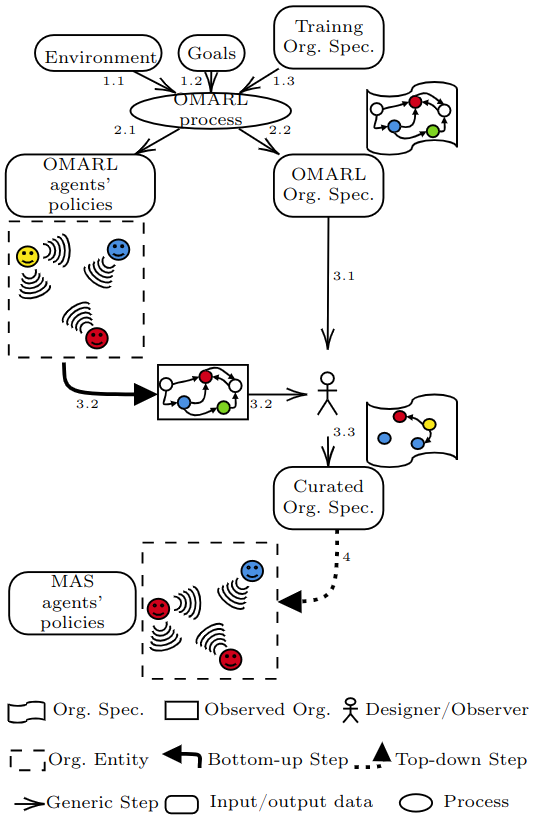
\includegraphics[width=1.2\linewidth]{figures/AOMEA_illustrative_view}
            }
        \end{column}
    
    \end{columns}
    
    \end{frame}    

\AtBeginSection[]{
    \begin{frame}
        \frametitle{}
        \tableofcontents[currentsection]
    \end{frame}
}

%%%%%%%%%%%%%%%%%%%%%%%%%%%%%%%%%%%%

\section{Evaluation in cooperative game environments}

\begin{frame}{Evaluation in cooperative game environments}

    \begin{block}{Atari-like environments}

        \begin{minipage}{0.5\textwidth}
            \centering
            \begin{itemize}
                \item \textquote{Drone swarm - 3rd CAGE Challenge}~\cite{cage_challenge_3_announcement} (CYB);
                \item \textquote{Pistonball} (PBL)~\cite{Terry2021};
                \item \textquote{Predator-prey with communication}~\cite{Lowe2017} (PPY);
                \item \textquote{Knights Archers Zombies}~\cite{Terry2021}.
            \end{itemize}
        \end{minipage}\hfill
        \begin{minipage}{0.5\textwidth}
            \centering
            \begin{figure}[H]
                \centering
                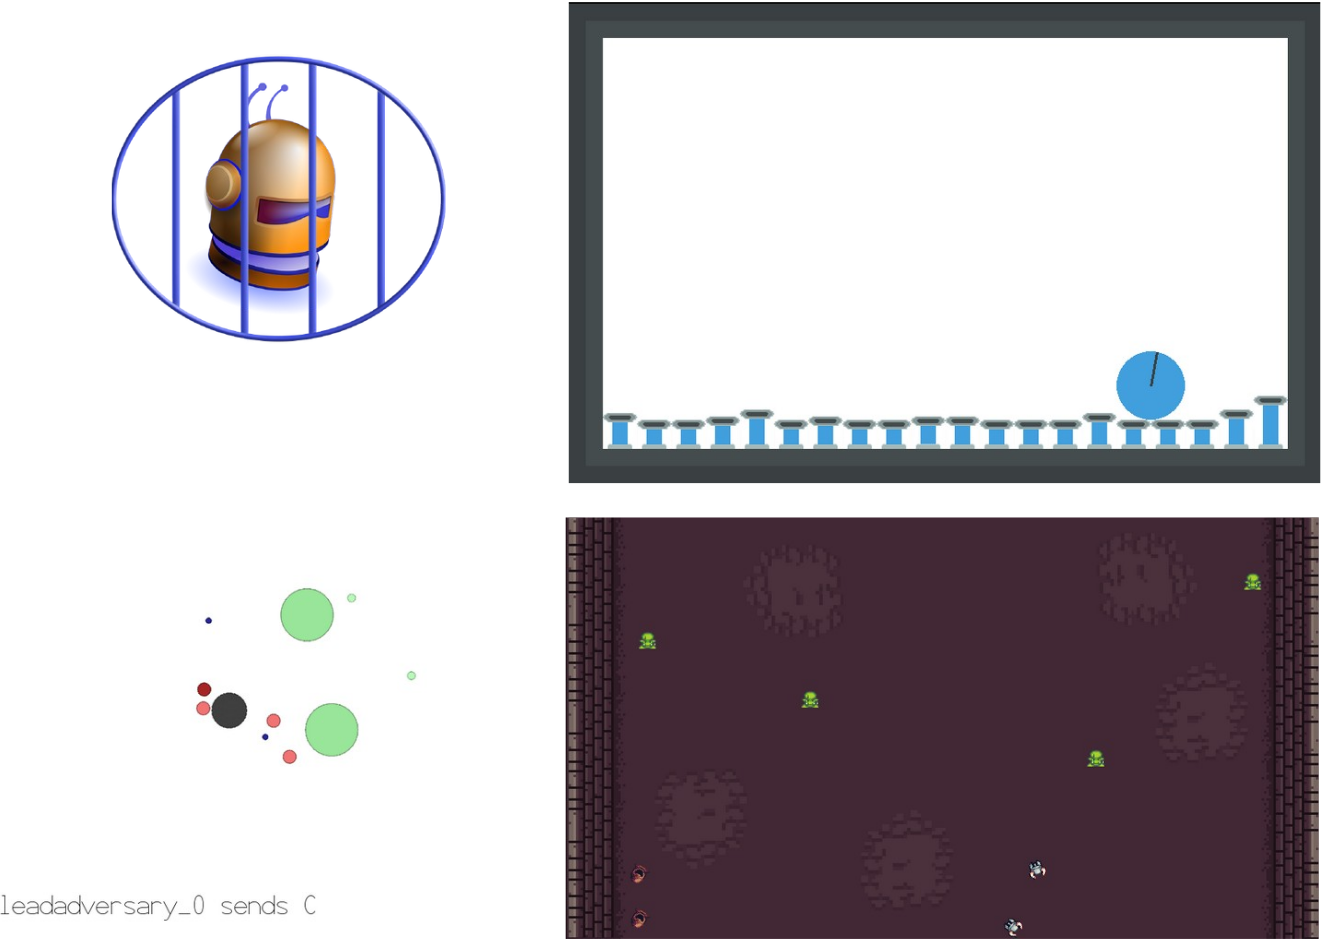
\includegraphics[width=0.5\linewidth]{figures/envs_4x4.png}
                \caption{Overview of the selected environments: CYB, PBL, PPY, and KAZ}
                \label{fig:simulated_environments}
            \end{figure}
        \end{minipage}\hfill

    \end{block}

    \begin{block}{Application modes of AOMEA}
        \begin{itemize}
            \item No organizational specifications (NTS)
            \item Partially constraining organizational specifications (PTS)
            \item Fully constraining organizational specifications (FTS)
        \end{itemize}
    \end{block}

    $\Longrightarrow$ Quantitative/qualitative assessment of performance impact during/after training

\end{frame}

\begin{frame}{Evaluation in cooperative game environments}{Some results}

    \begin{columns}

        \begin{column}{0.5\textwidth}
            \begin{figure}[h!]
                \centering
                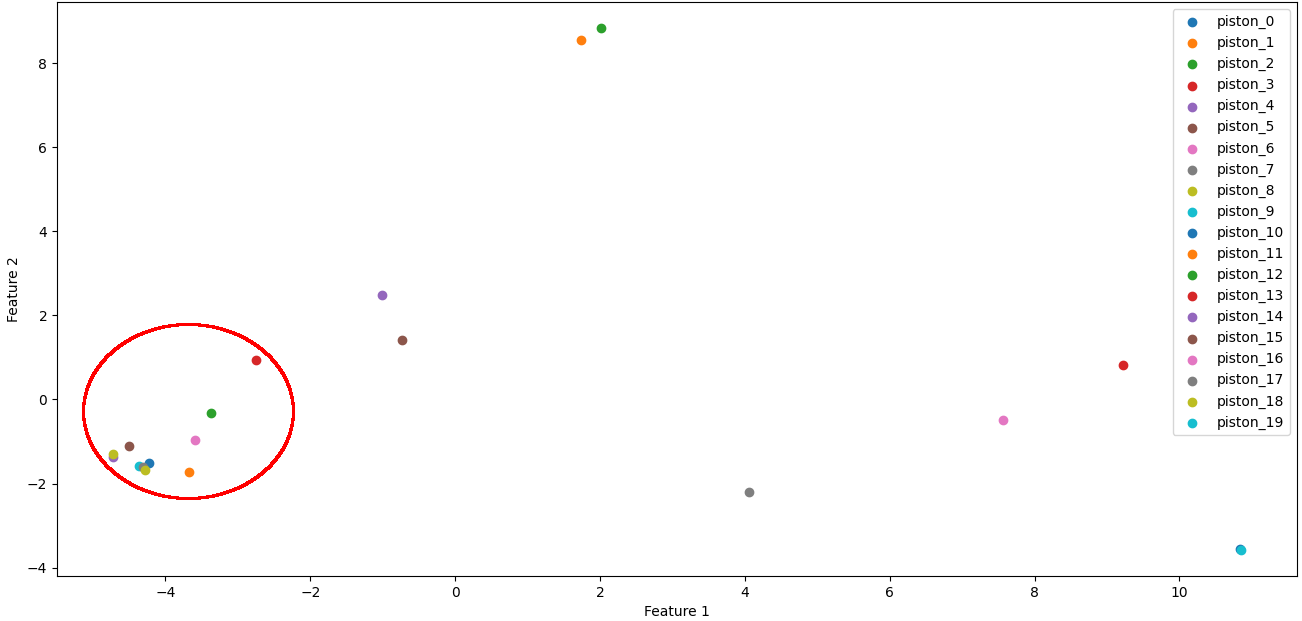
\includegraphics[width=\textwidth]{figures/prahom_pca_analysis.png}
                \caption{PCA of the trained agents' histories in the PBL environment}
                \label{fig:prahom_pca_analysis}
            \end{figure}
        \end{column}

        \hspace{1ex}

        \begin{column}{0.5\textwidth}
            \begin{figure}[h!]
                \centering
                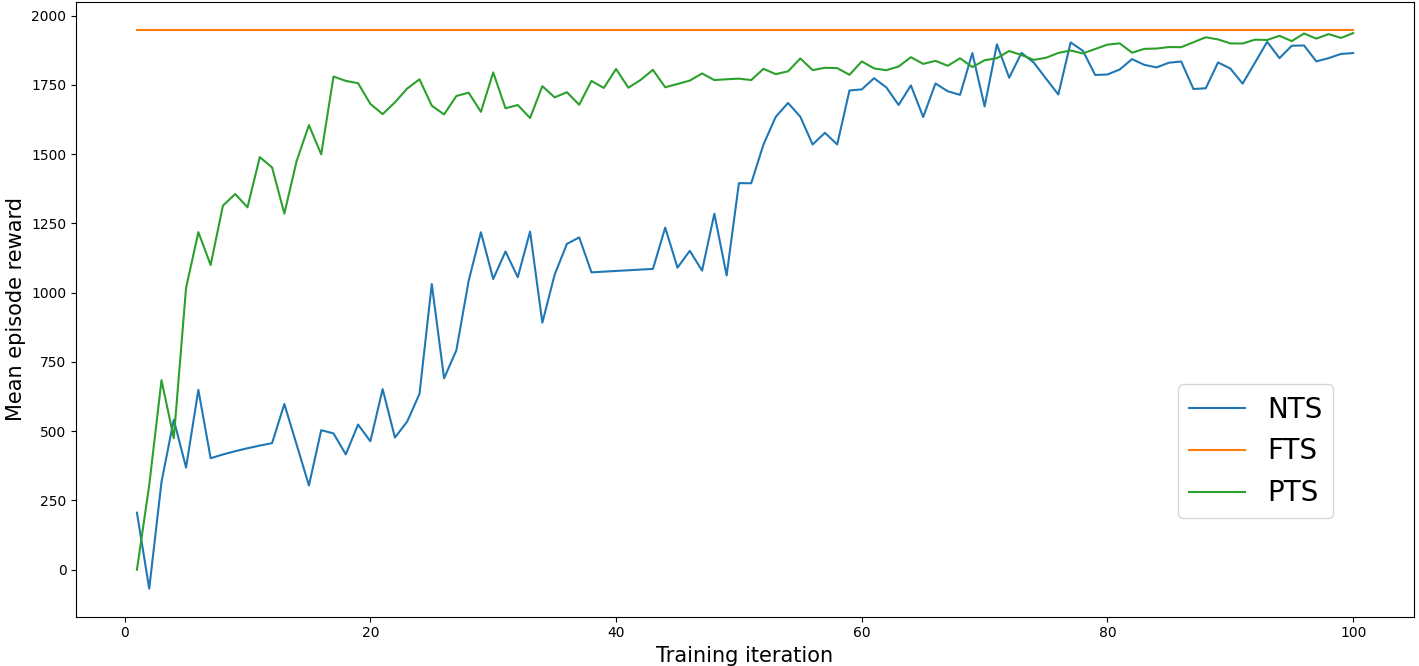
\includegraphics[width=0.95\textwidth]{figures/prahom_learning_curve.png}
                \caption{Average reward for each iteration in the PBL environment for the NTS, PTS, and FTS cases}
                \label{fig:prahom_learning_curve}
            \end{figure}
        \end{column}

    \end{columns}

\end{frame}

\begin{frame}{Evaluation in cooperative game environments}{Global discussion}

    \begin{block}{Performance impact during training}
        \begin{itemize}
            \item \textbf{Search space decreasing}: convergence time is longer for NTS than for PTS which is also longer than for FTS;
            \item \textbf{NTS outperformance}: trained agents' policies are hand-tailored to solve the problem;
            \item \textbf{Impact on solving strategy}: low-performance stability in CYB environment $\rightarrow$ no general strategies compared to the other environments.
        \end{itemize}
    \end{block}

    \begin{block}{Qualitative assessment of trained agents \& determined OS}
        \begin{itemize}
            \item \textbf{PBL}: share a common role $\rightarrow$ expected;
            \item \textbf{KAZ}: archers tend to move away from zombies, knights tend to approach them $\rightarrow$ two roles;
            \item \textbf{PPY}: authority links between the leader predator and the simple predators $\rightarrow$ collective strategies for circling prey
            \item \textbf{CYB}: communication links $\rightarrow$ isolate infiltrated drones or trying to fix and alert recently suspected drones.
        \end{itemize}
    \end{block}

\end{frame}

\section{Conclusion et perspectives}
\begin{frame}{Conclusion et perspectives}
    {}

    \begin{prosblock}{\textbf{Contribution fondamentale} : AOMEA}
        \textbf{AOMEA} : assistance conception avec MARL et un modèle organisationnel.
    \end{prosblock}

    \begin{prosblock}{\textbf{Contribution pratique} : PRAHOM}

        \begin{itemize}
            \item \emph{Wrapper PRAHOM PettingZoo} comme preuve de concept pour l'application pratique d'AOMEA ;
            \item Permet d'obtenir certaines OS (Organizational Specifications) qui satisfont les contraintes de conception et permettent d'atteindre des objectifs donnés.
        \end{itemize}

    \end{prosblock}

    \begin{alertblock}{Perspectives}
        \emph{PRAHOM} utilise les historiques pour reconstruire des comportements collectifs $\rightarrow$ \textbf{difficile}
        \begin{itemize}
            \item Rendre inférence de Spec. Org. plus robuste ;
            \item \textit{Simulation-to-reality gap} $\rightarrow$ Auto-encoder + LSTM pour modélisation environnement
            \item Explorer les travaux récents en MARL, tels que \textbf{l'apprentissage hiérarchique} ;
            \item LLM pour des descriptions textuelles complémentaires des OS définies par les historiques.
        \end{itemize}
    \end{alertblock}

\end{frame}


\appendix
%\setbeamertemplate{headline}{}
\setbeamertemplate{mini frames}{}

% \AtBeginSection[]{
% 	\begin{frame}
% 		\frametitle{}
% 		\tableofcontents[currentsection]
% 	\end{frame}
% }

% %%%%%%%%%%%%%%%%%%%%%%%%%%%%%%%%%%%%

\section*{\phantom{Thanks}}

\begin{frame}{}

  \vspace{6ex}

  \centering
  {
    \Huge
    \emph{Thank You}
  }

  \vspace{6ex}

  \begin{columns}

    \hspace{-27ex}

    \begin{column}{0.5\textwidth}
      \raggedleft
      {\Large Demo video $\Longrightarrow$}
    \end{column}

    \hspace{-12ex}

    \begin{column}{0.5\textwidth}
      
\includegraphics[width=0.5\linewidth]{figures/demo_qr_code.png}
    \end{column}

  \end{columns}

  \vspace{3ex}

  \centering
  {\Large
    \url{https://t.ly/4JBxr}
  }

\end{frame}

% \AtBeginSection[]{
% 	\begin{frame}
% 		\frametitle{}
% 		\tableofcontents[currentsection]
% 	\end{frame}
% }

% %%%%%%%%%%%%%%%%%%%%%%%%%%%%%%%%%%%%

\section*{\phantom{References}}

\begin{frame}[allowframebreaks]{References}{}
    
    % \bibliographystyle{plain}
    % \bibliography{local_references}
        
    \printbibliography

\end{frame}

\begin{frame}[allowframebreaks]{Annexes} {Contexte}

    \begin{block}{Paradigme des Systèmes Multi-Agents (SMA) pour des problèmes complexes et distribués}
        \begin{itemize}
            \item \textbf{décomposition des tâches} : missions déléguées aux agents réalisées par coopération~\parencite{Raileanu2023} ;
            \item \textbf{avantages} : gérer des objectifs contradictoires, calcul parallèle, robustesse du système, évolutivité\dots
        \end{itemize}
    \end{block}
    
    \begin{block}{\textbf{Organisation} : clé pour la conception des SMA}
        \begin{itemize}
            \item \textbf{coordination} : comment atteindre un objectif commun de manière collaborative~\parencite{Hubner2007} ;
            \item \textbf{environnements dynamiques et incertains} : comportement flexible à l'exécution pour s'adapter~\parencite{Kathleen2020} ;
        \end{itemize}
    \end{block}
    
    \begin{block}{Méthodes et pratiques pour la conception des SMA}
        \begin{itemize}
            \item \textbf{approche + modèle organisationnel} : les méthodes s'appuient sur l'expérience des concepteurs pour concevoir manuellement les \textbf{politiques} des agents afin que le SMA atteigne ses objectifs ;
                  %   \begin{itemize}
                  %       \item Exemples : \emph{GAIA}~\parencite{Wooldridge2000,Cernuzzi2014}, \emph{ADELFE}~\parencite{Mefteh2015}, ou \emph{DIAMOND}~\parencite{Jamont2015}, \emph{KB-ORG}~\parencite{Sims2008}
                  %   \end{itemize}
            \item \textbf{simulation vers la réalité} : 1) conception sûre et efficace des SMA dans un environnement simulé à haute fidélité ; \quad 2) transfert à un environnement réel pour des performances adéquates~\parencite{Schon2021}.
        \end{itemize}
        \quad $\Longrightarrow$ \textbf{Processus itératif par essais et erreurs}
    \end{block}

\end{frame}

\begin{frame}[allowframebreaks]{Annexes} {Fondamentaux des SMA}

    \begin{block}{Mots-clés}
        \begin{itemize}
            \item \textbf{Agent} : entité immergée dans un environnement, percevant des observations et prenant des décisions de manière autonome pour atteindre des objectifs ;
            \item \textbf{SMA} : ensemble d'agents collaborant avec des mécanismes d'auto/réorganisation pour atteindre leurs objectifs ;
            \item \textbf{Organisation} : interactions des agents même si elles peuvent être implicites ;
            \item \textbf{Modèle organisationnel (OM)} : moyen de décrire formellement une organisation explicite/implicite ;
            \item \textbf{Spécifications organisationnelles (OS)} : composants d'un OM pour caractériser une organisation.
        \end{itemize}
    \end{block}
    
    \begin{block}{Modèle organisationnel : $\mathcal{M}OISE^+$}
        \begin{itemize}
            \item plus complexe que \emph{Agent Group Roles} (intégration des normes) ;
            \item prend explicitement en compte les aspects sociaux entre les agents ;
            \item permet de lier les politiques des agents aux spécifications organisationnelles.
        \end{itemize}
    \end{block}

\end{frame}

\begin{frame}[allowframebreaks]{Annexes} {Fondamentaux du MARL}

    \begin{block}{Mots-clés}
        \begin{itemize}
            \item \textbf{Politique} : la \textquote{logique} pour choisir la prochaine action en fonction de l'observation pour un agent ;
            \item \textbf{Historique/trajectoire} : le couple (observation, action) sur un épisode ;
            \item \textbf{Politique/historique conjoints} : l'ensemble des politiques/historiques de tous les agents sous forme de tuples ;
            \item \textbf{Apprentissage par renforcement} : un agent met à jour sa politique pour maximiser une récompense cumulative ;
            \item \textbf{Apprentissage par renforcement multi-agent (MARL)} : extension à plusieurs agents qui apprennent en prenant en compte les actions des autres agents ;
        \end{itemize}
    \end{block}
    
\end{frame}

\begin{frame}[allowframebreaks]{Annexes}{Approche AOMEA : Fondement théorique}
    \begin{block}{MARL orienté organisation (OMARL)}
        Un processus de MARL augmenté avec un OM pour :
        \begin{itemize}
            \item \textbf{Contraindre l'espace des politiques} : obtenir les politiques conjointes satisfaisant les spécifications de conception données ;
            \item \textbf{Inférer des spécifications organisationnelles} : obtenir des spécifications à partir des politiques des agents.
        \end{itemize}
    \end{block}
    
    \begin{block}{Algorithme \emph{Partial Relations with Agent History and Organization Model} (PRAHOM)}
        Implémentation d'un processus OMARL\dots
        \begin{enumerate}
            \item \textbf{Contraindre l'espace des politiques}
                  \begin{itemize}
                      \item Impossible d'utiliser directement les politiques $\rightarrow$ \textbf{historiques} caractérisant les \textbf{politiques} ;
                      \item Relations entre \textbf{OS} et historiques attendus ;
                      \item Les agents contraints aux OS $\rightarrow$ à chaque étape : actions disponibles mises à jour en fonction des historiques \textbf{OS}.
                  \end{itemize}
    
            \item \textbf{Inférer des spécifications organisationnelles}
                  \begin{itemize}
                      \item Analyser les historiques $\rightarrow$ caractériser les comportements collectifs comme OS ;
                      \item Utilisation des relations connues entre OS et historiques ;
                      \item Utilisation de la définition générale des OS par rapport aux historiques.
                  \end{itemize}
        \end{enumerate}
    \end{block}
    
\end{frame}

\begin{frame}{Annexes}{Aperçu de \textit{PRAHOM}}
    \begin{figure}
        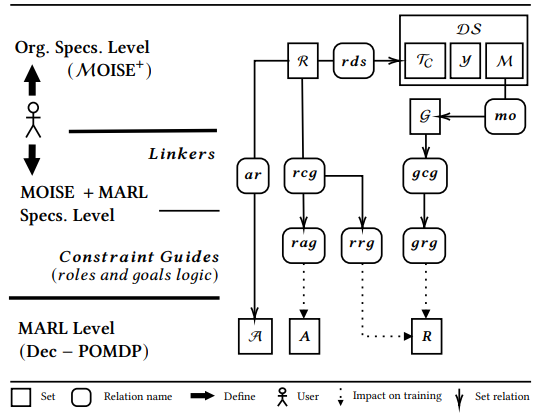
\includegraphics[width=0.6\linewidth]{figures/mm_simple_representation.png}
    \end{figure}
\end{frame}
    
\begin{frame}{Annexes}{Aperçu de PRAHOM}
    \begin{figure}
        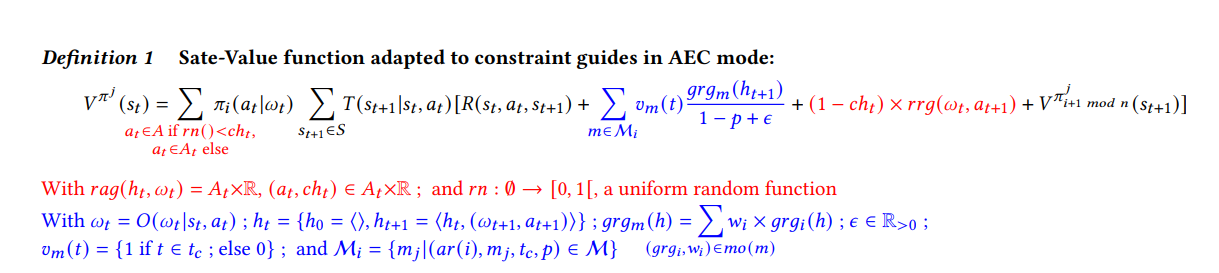
\includegraphics[width=\linewidth]{figures/modified_state_value_function.png}
    \end{figure}
\end{frame}
    
\begin{frame}[allowframebreaks]{Annexes}{Approche AOMEA : Fondement théorique}
    \textbf{Contraindre l'espace des politiques} pendant l'entraînement

    \begin{columns}
    
        \begin{column}{0.3\textwidth}
    
            \begin{itemize}
                \item À chaque étape, l'ensemble des actions disponibles est modifié pour correspondre aux contraintes de politiques définies par les utilisateurs ;
                \item Contraintes intégrées via : correction externe, apprentissage, modification interne des politiques.
            \end{itemize}
    
        \end{column}
    
        \begin{column}{0.8\textwidth}
            \begin{figure}
                \centering
                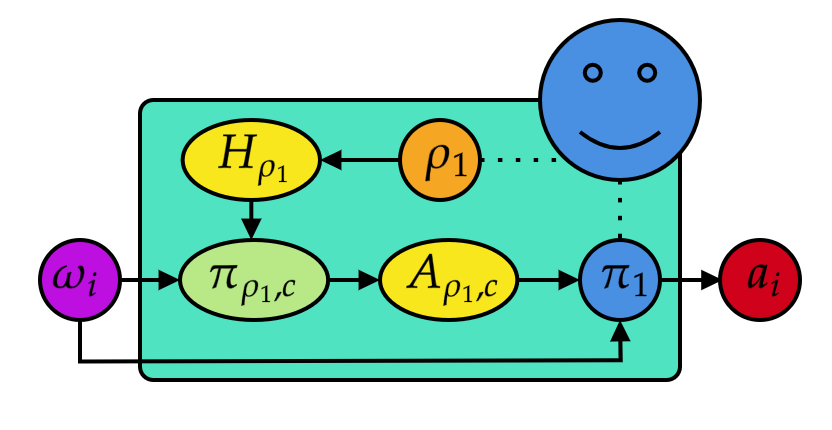
\includegraphics[width=0.7\linewidth]{figures/prahom_training_constrain.png}
                \caption*{Vue résumée de la contrainte PRAHOM}
                \label{fig:prahom_process}
            \end{figure}
        \end{column}
    
    \end{columns}
\end{frame}

\begin{frame}{Annexes}{Constrained Reinforcement Learning (Constrained-RL)}
    
    \begin{itemize}
        \item Apprendre une politique optimisant la récompense tout en respectant des \textbf{contraintes de sécurité} ou de \textbf{performance}.
        
        \item \textbf{Contraintes dures} : doivent toujours être respectées (Shielding).
        \item \textbf{Contraintes douces} : respectées en moyenne ou sous forme de pénalités.
        
        \item \textbf{Méthodes :}
            \begin{itemize}
                \item \textbf{Reward Shaping} : ajout de pénalités pour violation de contraintes.
                \item \textbf{Policy Projection} : ajustement des actions pour rester dans les limites.
                \item \textbf{Dual Variables} : intégration de multiplicateurs de Lagrange pour gérer les contraintes.
            \end{itemize}
            
    \end{itemize}    
\end{frame}

\begin{frame}{Annexes}{Safe Exploration et Shielding en Reinforcement Learning}
    
    \begin{itemize}
        \item \textbf{Safe Exploration} $\rightarrow$ garantir la sécurité lors de la phase d'exploration en limitant les risques de comportements dangereux.
        \item Principalement modifier la fonction de récompense (Langragien) pour integrer contraintes mais aussi\dots
        \item \textbf{Shielding} intervenir en temps réel pour bloquer les actions susceptibles de violer ces contraintes, permettant une exploration sécurisée.
    \end{itemize}
    
    \textbf{Référence :} \\
    \textit{Akifumi Wachi, Wataru Hashimoto, Xun Shen, \& Kazumune Hashimoto (2023). Safe Exploration in Reinforcement Learning: A Generalized Formulation and Algorithms. In Thirty-seventh Conference on Neural Information Processing Systems.}

\end{frame}

\begin{frame}[allowframebreaks]{Annexes}{Approche AOMEA: Fondement théorique}

    \textbf{Inferrer des Spécifications Organisationnelles}

    \begin{columns}

        \begin{column}{0.3\textwidth}

            \begin{itemize}
                \item \textbf{Knowledge-based Organizational Specifications Identification (KOSIA)}
                \item \textbf{General Organizational Specifications Infererence (GOSIA)}
            \end{itemize}

        \end{column}

        \begin{column}{0.8\textwidth}
            \begin{figure}
                \centering
                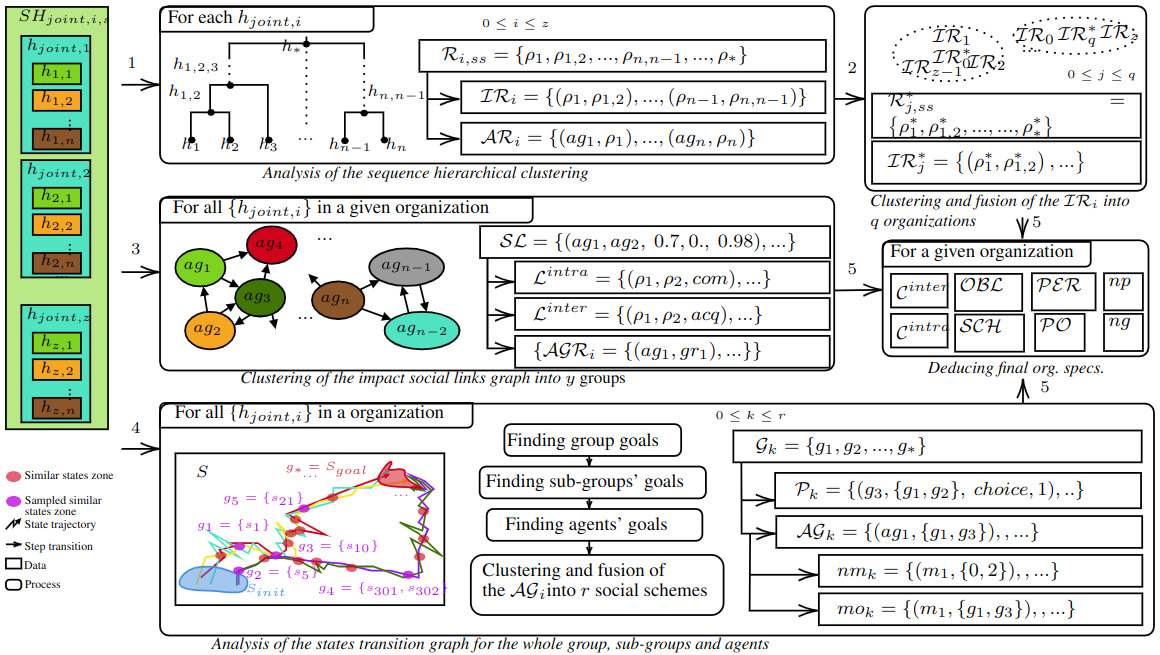
\includegraphics[width=0.95\linewidth]{figures/GOSIA_view.png}
                \caption*{A summary view of the GOSIA process}
                \label{fig:gosia_process}
            \end{figure}
        \end{column}

    \end{columns}

\end{frame}


%%%%%%%%%%%%%%%%

% Slide 2: Exemple d'utilisation
\begin{frame}[fragile]{Annexes}{Exemple d'utilisation d'Optuna}
    \begin{itemize}
        \item \textbf{Optuna} est une bibliothèque open-source pour l'optimisation des hyperparamètres (HPO), utile en apprentissage automatique.
        \item Exemples d'hyper-paramètre : taux d'apprentissage, fonction activation, nb couche, taille couches, seuil de ressemblance pour Hierarchical Clustering\dots
        \item \textbf{Étapes pour utiliser Optuna :}
        \begin{itemize}
            \item \texttt{1.} Définir une fonction d'objectif.
            \item \texttt{2.} Lancer une étude avec Optuna.
            \item \texttt{3.} Utiliser le meilleur résultat pour entraîner le modèle.
        \end{itemize}
    \end{itemize}

    \begin{lstlisting}[language=Python, basicstyle=\small\ttfamily, frame=single, caption=Exemple d'Optuna en Python]
import optuna

def objective(trial):
    x = trial.suggest_float("x", -10, 10)
    return (x - 2) ** 2 # Mock : fonction "etat-valeur"

study = optuna.create_study(direction="minimize")
study.optimize(objective, n_trials=100)

print(study.best_params)  # Affiche les meilleurs parametres
    \end{lstlisting}
\end{frame}


\begin{frame}{Annexes}{Aperçu PettingZoo}
    \begin{itemize}
        \item Bibliothèque Python pour environnements multi-agents.
        \item Simplifier l'entraînement et l'évaluation des agents dans divers environnements.
        \item \textbf{Caractéristiques principales} :
        \begin{itemize}
            \item Supporte plusieurs types d'environnements multi-agents (tour par tour, simultané, etc.).
            \item Intégration facile avec des frameworks de reinforcement learning comme RLlib.
            \item Compatible avec les API de Gym, permettant une utilisation intuitive.
        \end{itemize}
        \item \textbf{Exemples d'environnements inclus} :
        \begin{itemize}
            \item Jeux : \textit{TicTacToe}, \textit{ConnectFour}.
            \item Scénarios de collaboration et de compétition : \textit{Pistonball}, \textit{Prisoner's Dilemma}.
            \item Intégration avec la suite d'environnements Atari pour le multi-agent.
        \end{itemize}
    \end{itemize}
\end{frame}

\begin{frame}[fragile]{Annexes}{Exemple utilisation de PettingZoo}
    \begin{itemize}
        \item Exemple : Création et interaction avec un environnement.
        \item Chargement de l'environnement, réinitialisation et étapes d'interaction pour un agent.
    \end{itemize}
    \vspace{0.3cm}
    \begin{lstlisting}[language=Python, basicstyle=\ttfamily\small]
from pettingzoo.butterfly import pistonball_v6

# Creer et reinitialiser l'environnement
env = pistonball_v6.env()
env.reset()

# Boucle principale d'interaction
for agent in env.agent_iter():
    obs, reward, done, info = env.last()
    action = env.action_space(agent).sample()  # Action aleatoire
    env.step(action)
    if done:
        env.reset()  # Reinitialiser si l'episode est termine
\end{lstlisting}
\end{frame}


\begin{frame}{Annexes}{KB-Org}
    \frametitle{Organization-based multi-agent systems: From modeling to implementation}
    
    \begin{itemize}
        \item Modélisation et mise en œuvre des SMA basés sur organisation ;
        \item Intègre les concepts d'organisation pour structurer les interactions et le comportement des agents ;
        \item Banque d'organisations disponibles prêtes à être utilisé ;
        \item Explicabilité et à la coordination.
    \end{itemize}
    
    \

    Sims, V. (2008). Automated organization design for multi-agent systems. Autonomous Agents and Multi-Agent Systems, 16(2), 151-185.

\end{frame}

\begin{frame}{Annexes}{Présentation de la bibliothèque MARLlib}

    \begin{itemize}
        \item Bibliothèque Python pour MARL
        \item Supporte plusieurs environnements MARL comme PettingZoo, StarCraft II, MPE (Multi-Agent Particle Environment), etc.
        \item Implémente divers algorithmes MARL, incluant MADDPG, MAPPO, etc.
        \item Fournit une interface pour comparaison d’algorithmes, l’entraînement et l’évaluation.
        \item Offre des configurations \textit{fine-tunés} pour de nombreux environnements
    \end{itemize}

\end{frame}

\begin{frame}[allowframebreaks]{Annexes}{Présentation de la bibliothèque MARLlib}

    \begin{itemize}
        \item \textbf{Algorithmes Basés sur les Valeurs}  
        \begin{itemize}
            \item \textbf{Multi-Agent Q-Learning} : Une extension multi-agent fondamentale de Q-learning.  
            \textit{Description} : Simple à implémenter, mais avec des difficultés de scalabilité et de non-stationnarité.
            \item \textbf{MADDPG} : Une adaptation de DDPG pour les environnements multi-agents.  
            \textit{Description} : Gère bien les espaces d'actions continues, mais requiert beaucoup de données et est complexe.
        \end{itemize}
    
        \

        \item \textbf{Algorithmes Basés sur les Politiques}  
        \begin{itemize}
            \item \textbf{REINFORCE} : Une méthode de gradient de politique basique pour l'apprentissage direct de la politique.  
            \textit{Description} : Adaptable aux environnements stochastiques mais souffre de variances élevées des gradients.
            \item \textbf{Multi-Agent PPO (MAPPO)} : Une extension de PPO conçue pour les configurations multi-agents.  
            \textit{Description} : Stabilise les mises à jour, mais nécessite un ajustement minutieux et un coût de calcul élevé.
        \end{itemize}
    
        \item \textbf{Algorithmes Hybrides}  
        \begin{itemize}
            \item \textbf{A3C (Asynchronous Advantage Actor-Critic)} : Combine l'apprentissage des politiques et des valeurs pour un équilibre exploration/exploitation.  
            \textit{Description} : Accélère l'entraînement mais nécessite une synchronisation complexe.
            \item \textbf{MAPPO} : Un hybride intégrant PPO avec un entraînement centralisé.  
            \textit{Description} : Efficace pour les tâches coopératives, mais difficile dans les environnements compétitifs et exigeant en ressources.
        \end{itemize}
    
        \item \textbf{Algorithmes Théoriques et Coopératifs Basés sur le Jeu}  
        \begin{itemize}
            \item \textbf{Independent Q-Learning (IQL)} : Une version indépendante de Q-learning pour chaque agent.  
            \textit{Description} : Simple à implémenter mais avec de sérieux problèmes de non-stationnarité en multi-agent.
            \item \textbf{COMA (Counterfactual Multi-Agent Policy Gradients)} : Utilise des baselines contrefactuelles pour évaluer les contributions des agents.  
            \textit{Description} : Réduit la variance et améliore la coopération, mais demande des calculs lourds.
        \end{itemize}
    
        \item \textbf{Entraînement Centralisé avec Exécution Décentralisée}  
        \begin{itemize}
            \item \textbf{QMIX} : Décompose les valeurs Q pour améliorer la coordination multi-agent.  
            \textit{Description} : Équilibre l'entraînement centralisé et l'action décentralisée, mais moins efficace en environnements très compétitifs.
            \item \textbf{VDN (Value Decomposition Networks)} : Simplifie la coordination multi-agent avec la décomposition des valeurs.  
            \textit{Description} : Efficace mais limité dans la gestion d'interactions complexes.
        \end{itemize}
    \end{itemize}
    

\end{frame}

\end{document}
